\documentclass[brudnopis]{xmgr}
\usepackage{amsrefs}
\usepackage{mathtools}
\usepackage{ccaption}
\usepackage{amsthm}
\usepackage{todonotes}
\usepackage{placeins}
\usepackage{enumitem}

\DeclarePairedDelimiter\ceil{\lceil}{\rceil}
\DeclarePairedDelimiter\floor{\lfloor}{\rfloor}

\theoremstyle{definition}
\newtheorem{Twierdzenie}{Twierdzenie}
\newtheorem{Lemat}{Lemat} 
\newtheorem{Definicja}{Definicja} 

\wersja   {wersja wstępna [\ymdtoday]}

\author   {Jakub Ciechowski}
\nralbumu {186471}
\email    {jakubciechowski@gmail.com}

\title    {Problem galerii sztuki dla odcinków na płaszczyźnie}
\date     {\ymdtoday}
\miejsce  {Gdańsk}

\opiekun  {dr hab. Paweł Żyliński}

\begin{document}

% \begin{abstract}
%  Streszczenie…
% \end{abstract}
\keywords{Problem galerii sztuki}

\maketitle

\introduction
Jako pierwszy problem galerii sztuki przedstawił Victor Klee w 1973, odpowiadając na prośbę Vaseka Chv\'atala o interesujący problem geometryczny. Zagadnieniem, które zaproponował Klee było znalezienie minimalnej ilości strażników, wystarczających aby strzec wnętrze pomieszczenia galerii sztuki o kształcie $n$-kąta. Niedługo potem Chv\'atal zaproponował rozwiązanie tego problemu, które szybko zostało nazwane ,,Teorią galerii sztuki Chv\'atala''. Od tamtego dnia problem doczekał się wielu różnych wariacji oraz przekształceń. W pracy zajmę się rodziną problemów dotyczących odcinków na płaszczyźnie. 

Jednym z takich zagadnień jest strzeżenie zbioru odcinków, które wymaga aby strzeżony odcinek był widziany przez strażnika przynajmniej w jednym punkcie. Można to zobrazować przez stacjonarnych strażników, którzy, rozmieszczeni w odpowiednich punktach, zawsze widzą na przykład obraz, przez co uniemożliwiają zdjęcie go ze ściany. Innym ciekawym podejściem do sprawy strzeżenia odcinków jest ich oświetlanie, które  rozumiemy przez takie umieszczenie źródła światła aby każdy punkt należący do odcinka był widoczny z takiego źródła. Rozwiązaniem problemu jest zbiór źródeł światła które w całości oświetlają każdy odcinek należący do zbioru. 

Najbardziej nawiązującym do współczesności wariantem wywodzącym się z klasycznego problemu galerii sztuki jest zdecydowanie problem k-nadajników. Traktuje on strażników jako nadajnik o nieskończonym zasięgu oraz określonej mocy. Mając dany zbiór przeszkód oraz znając moc nadajników (tzn. liczbę przeszkód przez którą nadajnik jest w stanie nadawać) rozwiązanie problemu pozwala oszacować liczbę nadajników pozwalającą pokryć obszar, zawierający wszystkie przeszkody.

Kolejne zagadnienie wywodzące się z problemu galerii sztuki bazuje na zdegenerowanych wielokątach, a dokładnie na siatkach zarówno dwu jak i trójwymiarowych. Siatką nazywamy połączony ze sobą zbiór poziomych oraz pionowych odcinków prostych. Problem ten wymaga aby strażnik znajdował się w każdej z korytarzy siatki. Szacowanie liczby strażników dla siatek dwuwymiarowych ściśle wiąże się ze skojarzeniami w grafie natomiast dla siatek trójwymiarowych problem należy do klasy np-zupełnej.

Ostatni rozdział łączy w sobie klasyczny problem galerii sztuki oraz elementy z teorii grafów (?). Opisuje w nim wariant gry w policjanta i złodzieja, który wymaga aby policjant przemieszczający się z ograniczoną prędkością po krawędziach grafu zauważył złodzieja. Grafem jest siatka zdefiniowania podobnie jak we wcześniejszym problemie. Zakładamy, że policjant widzi przez całą długość krawędzi.


\chapter{Podstawowe pojęcia}

\begin{Definicja}{Wielokąt prosty}

  Płaska figura składające się z $n$ wierzchołków $v_1, v_2,\ldots, v_n$ oraz $n$ krawędzi $v_1v_2, v_2v_3, \ldots, v_{n-1}v_n,v_nv_1$ takich, że żadna para kolejnych krawędzi nie przecina się.
\end{Definicja}

\begin{Definicja}{Graf prosty}

  Zbiór $G = (V,E)$, gdzie $V$ jest niepustym skończony zbiorem wierzchołków a $E$ jest skończonym zbiorem krawędzi.
\end{Definicja}

\begin{Definicja}{Graf spójny}

  Graf którego nie można przedstawić jako sumy dwóch grafów.
\end{Definicja}

\begin{Definicja}{Odcinek prosty}

  Część prostej łącząca dwa punkty.
\end{Definicja}

\begin{Definicja}{Podgraf indukowany}

    asd
\end{Definicja}

\begin{Definicja}{Strażnik}

  Punkt $p$ na płaszczyźnie, który strzeże punktu $q$ wtedy i tylko wtedy jeżeli odcinek $\overline{pq}$ należy do wielokąta.
\end{Definicja}

\chapter{Klasyczny problem galerii sztuki}

\section{Twierdzenie Chv\'atala}
Zgodnie z twierdzeniem Chv\'atala (1975)\label{tw chvatala}, ilość strażników potrzebnych do strzeżenia wielokąta prostego $P$ wynosi $g(P) \le \floor{\frac{n}{3}}$, gdzie $g(P)$ jest funkcją opisującą ilość strażników wystarczających aby zawsze strzec określony $n$-kąt. Inaczej mówiąc, $g(P)$ strażników zawsze wystarcza a czasami jest potrzebnych aby pokryć $n$-kąt.
\\Przedstawię dowód Fiska (1978) powyższego twierdzenia, który jest znacznie prostszy od indukcyjnej wersji Chv\'atala, a który bazuje na trójkolorowaniu grafu. 

Pierwszym krokiem jest triangulacja wielokąta $P$, przez dodanie wewnętrznych przekątnych między wierzchołkami, do momentu gdy nie będzie można już dodać więcej krawędzi. 
Dowód na to, że każdy wielokąt prosty można podzielić na trójkąty, znajduje się w dodatku \ref{triangulacja}.
Za wierzchołki i krawędzie grafu przyjmujemy odpowiednio wierzchołki, krawędzie wielokąta oraz przekątne triangulacji. Jako że graf powstały po triangulacji jest planarny, zgodnie z twierdzeniem o czterech barwach (Appel i Haken, 1977) jest 4-kolorowalny.

\begin{Definicja}
   \it{$K$-kolorowanie grafu} to przyporządkowanie takiej liczby naturalnej każdemu wierzchołkowi grafu G, że żadnym dwóm sąsiednim wierzchołkom nie została przypisana taka sama liczba oraz wszystkie liczby są mniejsze bądź równe $K$.
\end{Definicja}

\begin{Lemat} \cite{fisk}
Graf wielokąta prostego po triangulacji zawsze jest $3$-kolorowalny.
\end{Lemat}
\begin{proof}
	Dowód polega na indukcji po ilości trójkątów wielokąta po triangulacji. Trójkąt jest przypadkiem bazowym -- zawsze można go pokolorować trzema kolorami. Następnym krokiem jest stworzenie grafu słabo dualnego dla grafu triangulacji danego wielokąta, który jest drzewem.
	\begin{figure}[ht!]
	  \centering
	  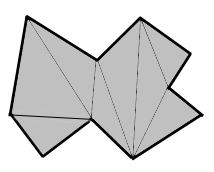
\includegraphics{rysunki/dual.png}
	    \caption{Wielokąt podzielony na trójkąty}
	\end{figure} 
	Z grafu dualnego usuwamy dowolny liść wraz z odpowiadającym mu ,,trójkątem'', kolorujemy wierzchołki grafu triangulacji, a następnie dodajemy trójkąt z powrotem nadając usuniętemu liściowi kolor inny niż sąsiadom.
	\begin{figure}[ht!]
	  \centering
	    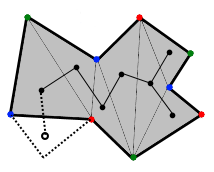
\includegraphics{rysunki/dual_kolor.png} 
	    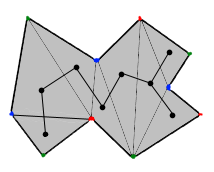
\includegraphics{rysunki/dual_caly_kolor.png}
	    \caption{Pokolorowany wielokąt wraz z grafem dualnym}
	\end{figure} 
	Strażników rozmieszczamy w tych wierzchołkach, których kolor jest najrzadziej używanym.
\end{proof}

\newpage\indent Ograniczenie $g(n) = \floor{\frac{n}{3}}$ nie oznacza, że wystarczy rozmieścić strażnika w co trzecim wierzchołku -- patrzy rysunek niżej.
\begin{figure}[ht!]
  \centering
  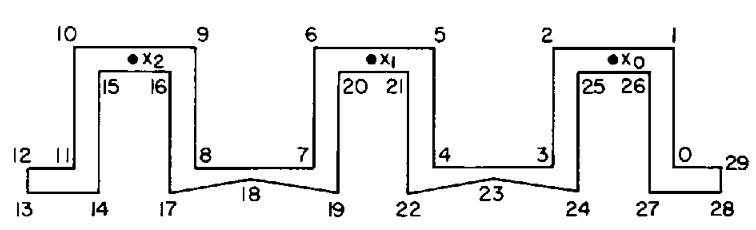
\includegraphics{rysunki/co_trzeci.png}
  \caption{Punkt $x$ jest niestrzeżony, przy rozmieszczeniu strażników w co trzecim wierzchołku.}
\end{figure} 

\section{Wielokąty z dziurami}
Ciekawym rozwinięciem klasycznego zagadnienia galerii sztuki jest wprowadzenie dziur do wnętrza wielokąta.

\begin{Definicja}\label{def wielokat z dziurami}
  \it{Wielokątem z dziurami} nazywamy wielokąt P, który mieści w sobie wiele innych wielokątów $H_1, \ldots, H_n$ nazywanych dziurami.
  Żaden wielokąt nie może przecinać zarówno krawędzi wielokąta $P$, jak i innych wielokątów wewnętrznych $H_i$.
\end{Definicja}

\indent Podobnie jak w przypadku standardowych wielokątów, również dla wariantu z dziurami, aby obliczyć potrzebną ilość strażników, wykorzystamy triangulację.

\begin{Lemat} \cite{orourke}
  Każdy wielokąt P z dziurami można podzielić na trójkaty.
\end{Lemat}

\begin{Lemat}\label{t trójkątów triangulacja} \cite{orourke}
  Każdy wielokąt P o \it{h} dziurach oraz \it{n} krawędziach poddany triangulacji, dzieli się na $t = n + 2h - 2$ trójkątów.
\end{Lemat}

W dowodzie skorzystam z twierdzenia Eulera.
\begin{Twierdzenie}\label{tw eulera}
  Niech G będzie spójnym grafem planarnym o N wierzchołkach, M krawędziach oraz F ścianach. Wówczas $N - M + F = 2$.
\end{Twierdzenie}

\begin{proof}
	Korzystając z tw. Eulera, mamy N wierzchołków, $F = t + h + 1$ ścian (po jednej na każdy trójkąt oraz dziurę i ścianę zewnętrzną), oraz $E = \frac{3t+n}{2}$ krawędzi (trzy krawędzie na każdy trójkąt plus krawędzie zewnętrzne liczone podwójnie).  Wówczas $V - E + F = 2$, a więc $n - \frac{3t+n}{2} + t + h + 1 - 2$, z czego wynika, że $t = n + 2h - 2$.
\end{proof}
Wiedząc, na ile trójkątów został podzielony wielokąt $P$, możemy przejść do twierdzenia określającego wymaganą ilość strażników.

\begin{Twierdzenie} \cite{orourke}
  Dla wielokąta o n wierzchołkach oraz h dziurach $\floor{\frac{n+2h}{3}}$ = $\ceil{\frac{t}{3}}$ strażników kombinatorycznych jest wystarczających, aby dominować każdą triangulację wielokąta.
\end{Twierdzenie}

\indent Główną ideą dowodu jest kolejne usuwanie dziur wielokąta, wzdłuż przekątnych dodanych podczas triangulacji, poprzez łączenie ich ze ścianą zewnętrzną. Każda z dziur posiada krawędź w grafie triangulacji $T$, która łączy ją z inną dziurą lub z zewnętrzną krawędzią wielokąta P. ,,Przecięcie'' wzdłuż takiej krawędzi połączy dziurę ze ścianą zewnętrzną lub scali dwie dziury w jedną. W każdym z tych przypadków całkowita ilość dziur zmniejszy się o jeden. Trudność polega jedynie na wyborze krawędzi z $T$, które pozwolą uzyskać taki podział.

\indent Niech $T'$ będzie grafem słabo dualny triangulacji $T$ (\ref{fig:triangulacja}). $T'$ jest grafem planarnym, co najwyżej stopnia trzy, posiadającym $h$ graniczących ze sobą scian $F_1, \ldots, F_h$, po jednej na każdą dziurę wielokąta P. Niech $F_0$ będzie ścianą zewnętrzną. Wybieramy dowolną ścianę $F_i$, która posiada przynajmniej jedną wspólną krawędź $e$ ze ścianą $F_0$. Taka krawędź istnieje, ponieważ w grafie $T$ musi istnieć przekątna łącząca krawędź zewnętrzną wielokąta $P$ z dowolną dziurą -- w grafie $T'$ jest to krawędź $e$. Usunięcie krawędzi $e$ z $T'$ scala $F_i$ z $F_0$, bez rozspójniania grafu.

\begin{figure}[h!]
  \centering
    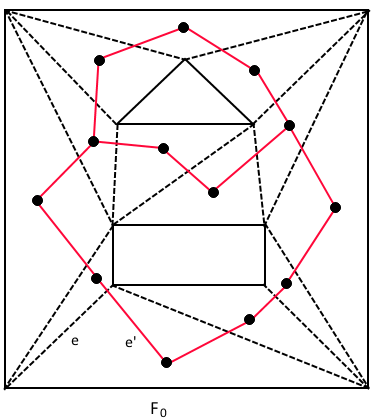
\includegraphics{rysunki/triangulacja_dziury.png}
    \caption{Wielokąt z dziurami wraz z grafem dualnym. Krawędź $e$ odpowiada krawędzi $e'$ w grafie dualnym.}
    \vspace{3in}
    \label{fig:triangulacja}
\end{figure} 

\indent Niech $P'$ będzie wielokątem uzyskanym według powyższej procedury. W takim wypadku $P'$ posiada $n + 2h$ krawędzi oraz $t$ trójkątów, ponieważ każde cięcie daje nam dwie dodatkowe krawędzie ale nie dodaje nowych trójkątów. Zgodnie z tw. Chv\'atala $P'$ potrzebuje co najwyżej $\floor{\frac{n+2h}{3}} = \ceil{\frac{t}{3}}$ strażników.

\chapter{Strzeżenie zbioru odcinków}
\section{Strzeżenie zbioru odcinków}
Ten wariant zagadnienia galerii sztuki wymaga, aby strzeżony odcinek był widoczny przez strażnika przynajmniej w jednym punkcie. 
\begin{Definicja}
Niech $F = \{S_1,\ldots,S_n\}$ będzie zbiorem $n$ prostych \it{odcinków} na płaszczyźnie. Zbiór punktów $Q = \{p_1,\ldots,p_k\}$ \it{strzeże} $F$, jeżeli każdy element $S_i$ ze zbioru $F$ zawiera punkt, który jest widziany przez przynajmniej jeden punkt $p_j$ należący do $Q$.
\end{Definicja}
Tak zdefiniowany problem możemy zobrazować przez strażników, którzy strzegą obrazu, jeżeli widzą tylko jego fragment. W takim przypadku nie można zdjąć obrazu ze ściany bez zaalarmowania strażnika.
\begin{figure}[ht!]
 \centering
  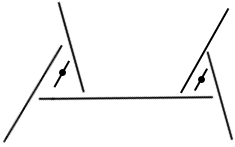
\includegraphics{rysunki/rozlaczny_dwoch_straznikow.png}
  \caption{Zbiór odcinków rozłącznych wymagający dwóch strażników}
\end{figure} 

\begin{Twierdzenie}\label{straznicy strzezenie} \cite{illumination}
Aby \it{strzec} dowolny zbiór $n$ \it{odcinków} prostych czasami potrzeba $\floor{\frac{2n-3}{5}}$, a zawsze wystarcza $\ceil{\frac{n}{2}}$ strażników.
\end{Twierdzenie}

\subsection{Ograniczenie górne}
Aby udowodnić twierdzenie \ref{straznicy strzezenie} na początku wykażemy, że dla każdego zbioru $F$ rozłącznych odcinków prostych, których jest parzysta liczba $n$, graf $G(F)$ ma doskonałe skojarzenie.
Rozpatrzmy teraz zbiór $F =\{S_1,\ldots,S_n\}$ rozłącznych odcinków prostych na płaszczyźnie oraz graf $G(F)$ zawierający $n$ wierzchołków $v_1$,\ldots,$v_n$ takich, że $v_i$ jest sąsiedni z $v_j$ wtedy i tylko wtedy, jeżeli istnieje punkt \textit{x} na płaszczyźnie, który widzi przynajmniej jeden punkt na odcinku $S_i$ i $S_j$ tzn. $x$ strzeże oba odcinki $S_i$ oraz $S_j$.

\begin{figure}[ht!]\label{zbior odcinkow rozlacznych}
 \centering
  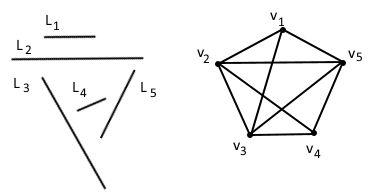
\includegraphics{rysunki/g_f.png}
  \caption{Zbiór $F$ odcinków rozłącznych oraz odpowiadający mu graf $G(F)$.}
\end{figure} 

\begin{Lemat}\label{podgraf indukowany} \cite{illumination}
Niech $Q$ będzie dowolnym wielokątem prostym, a $F = \{S_1,\ldots,S_n\}$ zbiorem n rozłącznych odcinków, oraz niech H będzie podzbiorem elementów F takich które przecinają wielokąt Q wówczas podgraf grafu $G(F)$ indukowany przez wierzchołki $G(F)$ reprezentujące elementy ze zbioru H jest spójny.
\end{Lemat}
\begin{figure}[ht!]
 \centering
  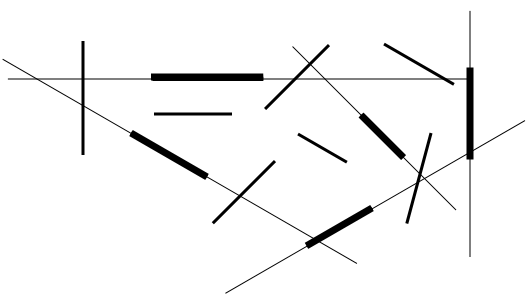
\includegraphics[height=3cm]{rysunki/podzial_h.png}
  \caption{Podział zbioru F. Pogrubione elementy należą do zbioru H}
\end{figure} 
Niech \textit{F} = \{$S_1$,\ldots,$S_n$\} będzie zbiorem $n$ rozłącznych odcinków, a $G(F)$ odpowiadającym mu grafem. Zakładamy, że $n$ jest parzyste, w przeciwnym wypadku należy dodać jeden odcinek do zbioru $F$. Pokażemy teraz, że $G(F)$ spełnia twierdzenie Tutte'a, a więc posiada skojarzenie doskonałe.
\begin{Definicja}
	Symbolem $o(G)$ oznaczamy liczbę składowych spójności grafu $G$, które posiadają nieparzystą liczbę wierzchołków.
\end{Definicja}
\begin{Twierdzenie} \cite{tutte}
	Spójny graf prosty $G$ posiada \it{doskonałe skojarzenie} wtedy i tylko wtedy, gdy dla każdego $S \subseteq V(G)$ zachodzi $o(G-S) \le |S|$.
\end{Twierdzenie}

\indent Rozważmy dowolny podzbiór $H$ zbioru $F$ oraz niech $S$ będzie zbiorem wierzchołków grafu $G(F)$ reprezentujących elementy $H$. Pokażemy, że liczba składowych spójności grafu $G(F) \setminus S$ wynosi co najwyżej |$S$| = |$H$|.
\\\indent Najpierw usuwamy (z płaszczyzny) wszystkie odcinki, które nie należą do \textit{H}. Następnie, jeden po drugim przedłużamy elementy $H$ dopóki nie przetną innego elementu $H$, wcześniej przedłużonego odcinka lub nie staną się prostymi bądź półprostymi. Niech $\pi$ oznacza płaszczyznę indukowaną przez przedłużone elementy zbioru $H$. Łatwo zauważyć, że $\pi$ zawiera dokładnie |$H$| + 1 ścian. 
\\\indent Zgodnie z lematem \ref{podgraf indukowany}, liczba składowych spójności grafu $G(F) \setminus S$ jest co najwyżej równa ilości ścian płaszczyzny $\pi$ czyli |$H$| + 1. Można ponadto wykazać, że występują przynajmniej dwie sąsiednie ściany z $\pi$ takie, że odcinki, które je przecinają, należą do tej samej składowej spójności w grafie $G(F) \setminus S$. Stąd wniosek, że liczba elementów zbioru $G(F) \setminus S$ wynosi co najwyżej |$S$|, co implikuje, że $G(F)$ ma doskonałe skojarzenie $M$. Na tej podstawie możemy stwierdzić, że wystarczy co najwyżej $\ceil{\frac{n}{2}}$ punktów aby strzec $F$ -- po jednym na każdy wierzchołek krawędzi skojarzenia $M$.
\subsection{Ograniczenie dolne}
\indent Aby uzyskać ograniczenie dolne, należy wskazać $n$-elementowy zbiór $F$, który wymaga $\floor{\frac{2n-3}{5}}$ strażników.
\\\indent Niech $H$ będzie planarnym grafem kubicznym z trójkątną ścianą zewnętrzną, w której wszystkie wierzchołki, poza zewnętrznymi, spełniają założenie, że wektory wychodzące z wierzchołków wzdłuż krawędzi rozpinają płaszczyznę. $H$ posiada $k$ wierzchołków, wtedy ma $\frac{3k}{2}$ krawędzi.
\\\indent Zamieńmy krawędzie zbioru $H$ na odcinki takie, że na każde $k - 3$ wewnętrzne wierzchołki przypada trójkątna ściana, w której umieszczamy mały odcinek (rys. \ref{fig:przeksztalcenie h}).
\begin{figure}[ht!]
 \centering
  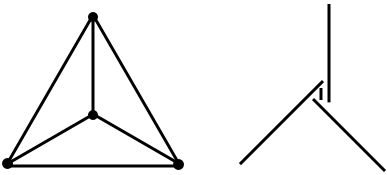
\includegraphics{rysunki/dolna_granica.png}
  \caption{Przekształcenie grafu H.}
  \label{fig:przeksztalcenie h}
\end{figure} 
Odrzucamy trzy krawędzie zewnętrznej ściany $H$, a następnie rozłączamy każdą krawędź w jej bliskim sąsiedztwie, tak aby utworzyć zbiór $n = (\frac{3k}{n}) - 3 + k  - 3$ odcinków. Żadne dwa z $k - 3$ małych odcinków nie są widoczne z jednego punktu więc $k - 3$ punktów jest potrzebnych aby strzec taki zbiór. Możemy łatwo sprawdzić, że $k - 3$ punktów jest również wystarczające gdyż $k - 3 = \floor{\frac{2n - 3}{5}}$, co kończy dowód twierdzenia \ref{straznicy strzezenie}.

\section{Oświetlanie odcinków}\label{oświetlanie odcinków}
Kolejną wariacją strzeżenia odcinków jest ich oświetlanie. Tym razem aby strzec odcinek, wymagane jest jego oświetlenie.
\begin{Definicja}
	Zbiór źródeł światła S \it{oświetla} zbiór odcinków prostych F wtedy i tylko wtedy, jezeli każdy punkt leżący na odcinku ze zbioru F \it{jest widzialny} z co najmniej jednego elementu z S.
\end{Definicja} Należy zwrócić uwagę na fakt, że punkt na odcinku może zostać oświetlony przez promień padający na niego z dowolnej strony odcinka.

\begin{Twierdzenie} \cite{illumination}
 Dowolny zbiór F składający się z n rozłącznych odcinków możemy oświetlić przy użyciu co najwyżej $\ceil{\frac{2n}{3}} - 3$ źródeł światła
\end{Twierdzenie}

\subsection{Ograniczenie górne}
\indent Niech $F$ = \{$L_1, \ldots, L_n$\} będzie zbiorem $n$ rozłącznych odcinków. Niech $T$ będzie trójkątem, który zawiera wewnątrz wszystkie elementy ze zbioru $F$ oraz niech $F'$ będzie zbiorem zawierającym elementy $F$ oraz trzy odcinki $L_{n+1}$, $L_{n+2}$, $L_{n+3}$ uzyskane przez skrócenie boków trójkąta $T$ o $\epsilon$ $>$ 0
Następnie, niech $H$ = \{$S_1,\ldots,S_n,S_{n+1},S_{n+2},S_{n+3}$\} będzie rodziną zbiorów złożoną z $n + 3$ ściśle wypukłych oraz wzajemnie wewnętrznie rozłącznych zbiorów (zbiory mogą się stykać tylko w jednym punkcie -- na ich granicach) spełniającą następujące założenia.
\begin{enumerate}
  \item $L_i$ zawiera się w $S_i$, gdzie $i = 1,\ldots,n+3$.
  \item Liczba punktów w których para elementów rodziny H styka się jest maksymalna
\end{enumerate}
\begin{figure}[ht!]
 \centering
  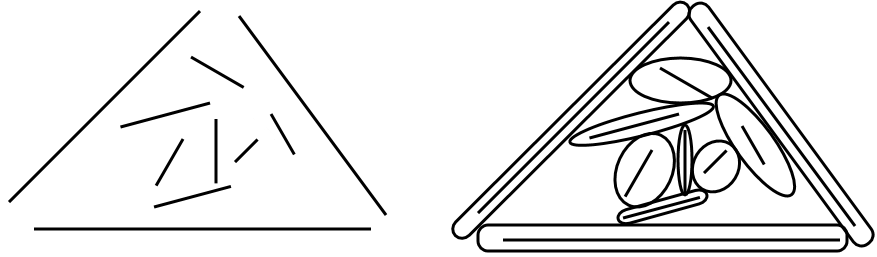
\includegraphics[height=5cm, width=13.5cm]{rysunki/podswietlenie.png}
  \caption{Zbiór $F'$ i rodzina $H$ zbiorów.}
\end{figure} 
Możemy łatwo zauważyć, że elementy rodziny $H$ są styczne z przynajmniej trzeba innymi elementami z tego zbioru. 
\\\indent Kolejnym krokiem jest stworzenie grafu $G$ poprzez zamianę każdego elementu zbioru $H$ na wierzchołek, przy założeniu, że dwa wierzchołki są sąsiednie, jeżeli odpowiadające im zbiory są styczne.
\begin{figure}[ht!]
 \centering
  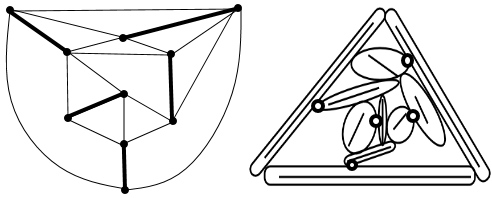
\includegraphics[height=4cm]{rysunki/skojarzenia_zrodla_swiatla.png}
  \caption{Graf G oraz źródła światła}
\end{figure}
Tak stworzony graf jest planarny oraz 2-spójny. Jako że każdy zbiór rodziny $H$ jest styczny z co najmniej trzema innymi zbiorami, stopień każdego wierzchołka grafu $G$ wynosi co najmniej trzy. Zgodnie z twierdzeniem Nishizaki (1977) dla grafu $G$ istnieje skojarzenie M o mocy co najmniej $\ceil{\frac{(n+3)+4}{3}} = \ceil{\frac{n+1}{3}}  + 2$. Dla każdej pary elementów $S_i$ i $S_j$ skojarzonych w $M$ przez krawędź $G$, należy teraz umieścić źródło światła w punkcie ich styczności. W tak wyznaczonym punkcie światło będzie oświetlać odcinki $L_i$ oraz $L_j$ zawierające się, odpowiednio, w $S_i$ oraz $S_j$. Jako że skojarzenie $M$ ma przynajmniej $\ceil{\frac{n+1}{3}} + 2$ elementów, $2(\ceil{\frac{n+1}{3}} + 2)$ elementy ze zbioru $F$ pokryta zostaną przez $\ceil{\frac{n+1}{3}} + 2$ świateł. W każdym z pozostałych elementów, które nie miały skojarzenia, musimy rozmieścić po jednym źródle. W rezultacie uzyskujemy:
$(\ceil{\frac{n+1}{3}} + 2) + ((n + 3) - 2(\ceil{\frac{n+1}{3}})) = n + 5 - \ceil{\frac{n+1}{3}} \le \ceil{\frac{2n}{3}} + 3$

\subsection{Ograniczenie dolne}
\indent Granica dolna nie jest dokładna. Przykładem zbioru dla którego potrzeba $\floor{\frac{2n-3}{5}}$ źródeł światła jest np. ten z rysunku \ref{fig:przeksztalcenie h} ze źródłem światła umieszczonym na wewnętrznym odcinku.

\subsection{Luka między ograniczeniem górnym a dolnym}
Z racji dużej różnicy pomiędzy ograniczeniem górnym a dolnym, znalezienie dokładnego wyniku wciąż jest problemem otwartym. Do tej pory nie udało się znaleźć dowodu chociażby na ograniczenie $\ceil{\frac{n}{2}}$ + c, gdzie \textit{c} jest stałą.

\section{Ukrywanie się za ścianami}
Po raz pierwszy problem ten przedstawili Hurtado, Serra oraz Urrutia (1996). Zdefiniowali oni problem w następujący sposób.

\begin{Definicja}\label{ukrywanie definicja}
 Rozpatrzmy zbiór rozłącznych odcinków $F$. Zbiór punktów $P$ nazywamy \textit{ukrytym} w stosunku do $F$, jeżeli dowolna prosta łącząca dwa punkty ze zbioru $P$ przecina element zbioru $F$.
\end{Definicja}

\begin{Twierdzenie}\label{podciag rosnacy} \cite{illumination}
  W każdym ciągu n liczb istnieje podciąg o długości co najmniej $\sqrt{n}$, rosnący lub malejący.
\end{Twierdzenie}

Dla tak zdefiniowanego problemu, korzystając z twierdzenia Erdosa i Szekeresa, uzyskali oni dokładne ograniczenie przez $\sqrt{n}$.
\begin{Lemat}\label{moc zbioru ukrytego tw} \cite{illumination}
  Dowolna rodzina n rozłącznych odcinków posiada zbiór punktów ukrytych o mocy co najmniej $\sqrt{n}$.
\end{Lemat}

Rozpatrzmy zbiór $F = \{L_1,\ldots,L_n\}$ odcinków takich, że ich rzut na oś OX tworzy rozłączny zbiór. Przez $\alpha_i$ oznaczamy nachylenie $L_i, i = 1,\ldots,n$ w stosunku do osi OX.
\begin{Lemat}\label{zbior ukryty}
  Jeżeli $\alpha_1 < \alpha_2 < \ldots < \alpha_n$ to $F$ posiada ukryty zbiór rozmiaru $n$.
\end{Lemat}

\begin{proof}
	Dla każdego odcinka $L_i$ niech punkt $p_i$ będzie jego środkiem. Wybierzmy punkt $q_i$, poniżej $p_i$, w niewielkiej odległości $\epsilon$ od $L_i$, \textit{i} = 1,\ldots,n. Rozpatrzmy dwie liczby całkowite \textit{i} $<$ \textit{j} oraz odcinek $L_{ij}$ łączący $p_i$ z $p_j$. Jeżeli $\alpha_i$ jest mniejsze niż nachylenie $\alpha_{ij}$ odcinka $L_{ij}$, wtedy wybierając $\epsilon$ wystarczająco małe, gwarantujemy, że odcinek łączący $q_i$ z $q_j$ przecina $L_i$. Jeżeli $\alpha_i$ jest większe lub równe $\alpha_{ij}$ to odcinek łączący $q_i$ z $q_j$ przetnie $L_j$. Obrazuje to rysunek \ref{fig:5 zbior ukryty}. A zatem, jeżeli $\epsilon$ jest dostatecznie małe to  $q_1, \ldots, q_n$ tworzy zbiór ukryty. 
\end{proof}
\begin{figure}[ht!]
  \centering
   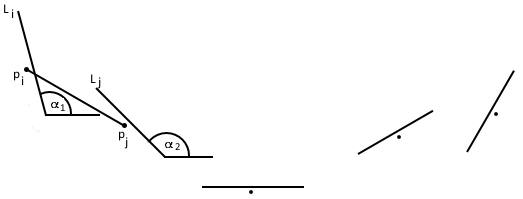
\includegraphics{rysunki/5_odcinkow_zbior_ukryty.png}
   \caption{Zbiór 5 odcinków o rosnącym nachyleniu, który posiada zbiór ukryty o rozmiarze równym 5.}
   \label{fig:5 zbior ukryty}
\end{figure}
\indent Przejdźmy teraz do właściwego dowodu twierdzenia \ref{moc zbioru ukrytego tw}. Rozpatrzmy rodzinę $n$ rozłącznych odcinków. Wybierzmy punkt $p_i$ na każdym z odcinków $L_i$ w taki sposób aby odcięte punktów $x_1,\ldots, x_n$ dla $p_i,\ldots,p_n$ były różne. Możemy założyć bez straty ogólności, że $x_1$ $<$ $x_2$ $<$ \ldots $<$ $x_n$. Następnie dla każdego $L_i$ wybierzmy odcinek $L'_i$ zawierający się w nim, ze środkiem w punkcie $p_i$, w taki sposób, że rzuty $L'_i,\ldots,L'_n$ na oś OX, tworzą zbiór rozłączny. Rozważmy teraz ciąg nachyleń $L'_1$, \ldots, $L'_n$. Zgodnie z def. \ref{podciag rosnacy} taki ciąg zawiera podciąg rosnący lub malejący o rozmiarze co najmniej $\sqrt{n}$, co biorąc pod uwagę lemat \ref{zbior ukryty}, kończy dowód twierdzenia \ref{moc zbioru ukrytego tw}.

\chapter{K-nadajniki}

\section{Pokrycie płaszczyzny z przeszkodami}
	Ilość sieci wi-fi cały czas rośnie, zarówno w naszych domach jak i w miejscach ogólnodostępnych. Fabila-Monroy oraz Aichholzer zainspirowani postępującą technologią przedstawili nowy problem, ściśle związany z teorią galerii sztuki. Opracowany przez nich wariant, nazywany ,,oświetleniem modemowym'', definiuje strażnika jako bezprzewodowy \textit{nadajnik} o nieskończonym zasięgu oraz możliwości przebicia $k$ ,,ścian''. Ściany są zazwyczaj reprezentowane przez odcinki na płaszczyźnie. Problem zdefiniowali następująco.
\textit{Mając dany zbiór przeszkód na płaszczyźnie, liczbę naturalną k $>$ 0 oraz dany obszar, jak wiele  nadajników jest potrzebnych oraz koniecznych, aby pokryć cały obszar?}  
\\\indent Warto zauważyć, że zagadnienie dla 0-nadajników to klasyczny problem galerii sztuki (strażnicy, którzy nie widzą przez ściany).
\\W wypadku, gdy wymagamy strzeżenia całej płaszczyzny, zakładamy, że nadajnik możemy umieścić wewnątrz ściany, co pozwala nadawać po jej obu stronach.
\subsection{Odcinki prostopadłe}
W tym podrozdziale omówię wariant, w którym przeszkodami będzie zbiór $n$ rozłącznych odcinków prostopadłych, a celem będzie pokrycie całej płaszczyzny. Czyżowicz i inni dowiedli, że $\ceil{\frac{n+1}{2}}$ 0-nadajników zawsze wystarcza, a czasami jest koniecznych, aby pokryć całą płaszczyznę, na której znajduje się $n$ rozłącznych prostopadłych odcinków. Ballinger i inni rozszerzyli to ograniczenie dla \textit{k-nadajników.}

\begin{Twierdzenie} \label{ograniczenie zbiór odcinków prostopadłych} \cite{knadajniki}
  $\ceil{\frac{5n+6}{12}}$ 1-nadajników jest zawsze wystarczających a $\ceil{\frac{n+1}{4}}$ czasami koniecznych aby pokryć całą płaszczyznę z n rozłącznymi odcinkami prostopadłymi.
\end{Twierdzenie}
\indent W oparciu o rysunek \ref{fig:ogr_dolne} łatwo wykazać dolną granicę ponieważ, pojedynczy 1-nadajnik może pokryć co najwyżej cztery z $n + 1$ obszarów, z czego wynika, że potrzebujemy $\ceil{\frac{n+1}{4}}$ 1-nadajników dla $n$ lini równoległych.
\begin{figure}[ht!]
  \centering
  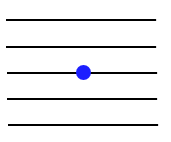
\includegraphics{rysunki/k_nadajniki_ogr_dolne.png}
  \caption{1-nadajnik strzegący 4 obszarów}
  \label{fig:ogr_dolne}
\end{figure} 
\\\indent Ograniczenie górne uzyskamy korzystając z następującego algorytmu:
\begin{itemize}
  \item ze zbioru wszystkich odcinków $S$ usuń odcinki ,,niezależne'';
  \item rozmieść 0-nadajniki;
  \item zwiększ zasięg przekaźników o jeden.
\end{itemize}

W pierwszym kroku przedłużamy wszystkie odcinki sekwencyjnie, dopóki się nie przetną lub nie staną się półprostymi, jednocześnie dzieląc płaszczyznę na $n + 1$ ścian. Następnie tworzymy graf widzialności $G(S)$, w którym każdy odcinek ze zbioru $S$ jest wierzchołkiem grafu. Krawędzie między wierzchołkami $s$ i $t$ tworzymy, jeżeli dwa odcinki $s$ i $t$ są słabo widzialne, tzn. istnieją punkty $p$ należący do odcinka $s$ oraz $q$ należący do odcinka $t$ taki, że odcinek $\overline{pq}$ nie przecina żadnego innego odcinka ze zbioru $S$.

\begin{Lemat}\label{0-1-nadajniki} \cite{knadajniki}
  Jeżeli $I$ jest niezależnym zbiorem w grafie $G(S)$, a $T$ jest zbiorem 0-nadajników, które pokrywają całą płaszczyznę ze zbiorem przeszkód $S \setminus I$, to $T$ jest również zbiorem 1-nadajników, które pokrywają całą płaszczyznę ze zbiorem przeszkód $S$
\end{Lemat}

\indent Załóżmy, że 0-nadajnik w punkcie $p$ pokrywa punkt $q$ na płaszczyźnie $S \setminus I$. Odcinek $\overline{pq}$ nie może przecinać dwóch lub więcej odcinków ze zbioru $I$, ponieważ wtedy takie odcinki nie byłyby niezależne. Jednocześnie, odcinek $\overline{pq}$ nie przecina żadnego odcinka ze zbioru $S \setminus I$ a więc 1-nadajnik w punkcie $p$ pokrywa $q$ na płaszczyźnie $S$.
\\\indent Aby uzyskać największy możliwy zbiór niezależny w $G(S)$, kolorujemy wierzchołki grafu $G(S)$ a następnie wybieramy najliczniejszą klasę kolorów. Zakładamy, że ściany powstałe przez przedłużenie odcinków w zbiorze \textit{S} są prostokątne (gdyby były trójkątne to graf $G(S)$ byłby planarny a więc 4-kolorowalny). 
Tak powstały graf jest 1-planarny oraz 6-kolorowalny (Ringel, 1965).

\begin{Definicja}
  Grafem 1-planarnym nazywamy graf, którego każda z krawędzi może przeciąć inną krawędź co najwyżej raz.
\end{Definicja}
\begin{figure}[ht!]
  \centering
  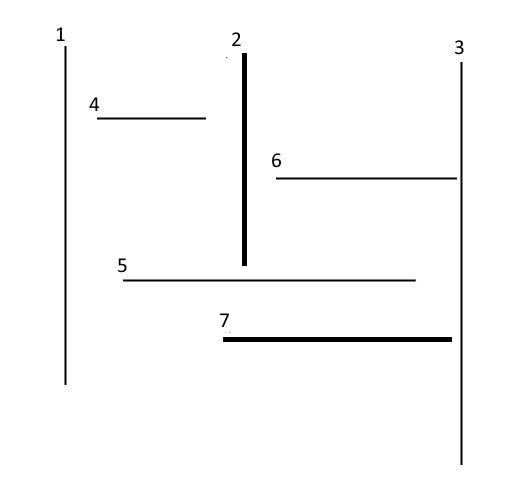
\includegraphics[width=6.5cm]{rysunki/zbior_odcinkow.png}
  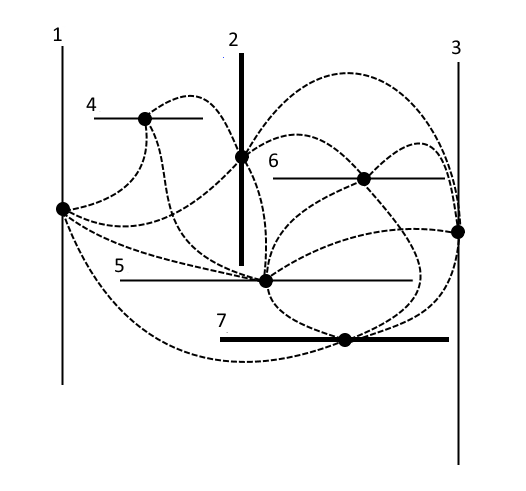
\includegraphics[width=6.5cm]{rysunki/graf_zbioru_odcinkow.png}
  \caption{Zbiór odcinków S oraz graf G(S). Zbiór niezależny został pogrubiony.}
  \label{fig:przedluzone odcinki}
\end{figure} 

\begin{Lemat} \cite{knadajniki}
  Jeżeli S jest zbiorem przedłużonych odcinków prostopadłych, to G(S) jest \textit{1-planarny}.
\end{Lemat}

\indent Aby uzyskać ograniczenie górne, kolorujemy graf $G(S)$ sześcioma kolorami. Najliczniejsza klasa kolorów ma więc nie mniej niż $\frac{n}{6}$ elementów oraz tworzy zbiór niezależny $I$. Pozostały zbiór $S \setminus I$ posiada $\frac{5n}{6}$ odcinków a więc zgodnie z rezultatem Czyżowicza wystarczy co najwyżej $\ceil{\frac{\frac{5n}{6} + 1}{2}}$ = $\ceil{\frac{5n+6}{12}}$ 0-nadajników, rozmieszczonych na odcinkach zbioru $S \setminus I$o tym samym kolorze. Następnie, zgodnie z lematem \ref{0-1-nadajniki}, zwiększamy moc rozmieszczonych nadajników o jeden, co pozwala strzec całą płaszczyznę.
\begin{figure}[ht!]
  \centering
  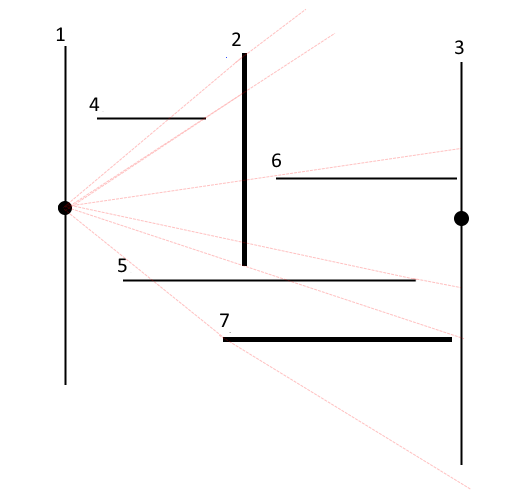
\includegraphics[width=6.5cm]{rysunki/pokrycie_nadajnikami.png}
  \caption{Pokrycie płaszczyzny 1-nadajnikami.}
  \label{fig:pokrycie plaszczyzny}
\end{figure} 

\section{Podział gilotynowy}
Podział gilotynowy $S$ otrzymujemy przez dodanie kolekcji $s_1,\ldots,s_n$ odcinków prostych w taki sposób, że każdy dodany odcinek $s_i$ dzieli dowolną ścianę podzbioru $S_{i-1}$ na dwie nowe ściany tworząc nowy podział $S_i$. Ścianą $S_0$ nazywamy całą płaszczyznę.

\begin{Lemat}\label{sasiednie sciany strzega F} \cite{knadajniki}
  Niech F będzie ścianą podziału gilotynowego S. Jeżeli każda inna ściana, która dzieli krawędź z F, posiada wewnątrz 1-nadajnik, to taki zbiór nadajników pokrywa całe F.
\end{Lemat}
\indent Rozpatrzmy odcinek $s_i$, którego dodanie tworzy ścianę $F$. Przed dodaniem odcinka $s_i$, podział $S_{i-1}$ zawierał jedną ścianę, która została podzielona na dwie części $F$ oraz $F'$ przez $s_i$. 
% \begin{figure}[ht!]
%   \centering
%   \label{podzial F przez s_i}
%   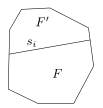
\includegraphics[width=9cm,height=6cm]{rysunki/podzial_F.png}
%   \caption{Ściana F oraz F' po dodaniu odcinka $s_i$}
% \end{figure} 


W dalszym procesie ściana $F$ nie będzie już dzielona, ale podzielimy ścianę F' uzyskujac kolejne ściany $F'_1$, \ldots, $F'_k$, takie, że $F'_j$ $\subseteq F'$ oraz $F'_j$ dzieli część odcinka $s_i$ ze ścianą $F$ dla każdego $j \in \{1,\ldots,k\}$

\begin{figure}[ht!]
  \centering
  \label{podzial F' na kolejne ściany}
  \includegraphics[width=9cm,height=6cm]{rysunki/podzial_F'.png}
  \caption{Kolejne podziały ściany F'}
\end{figure} 
Zgodnie z lematem \ref{sasiednie sciany strzega F} 1-nadajniki umieszczone wewnątrz ścian $F'_1, \ldots, F'_k$ strzegą wnętrza $F$. 
\\Aby to udowodnić, tymczasowo usuńmy odcinek $s_i$. W ten sposób uzyskalismy podział $S'$, przedłużając odcinki, którymi wcześniej dokonaliśmy podziału ściany $F'$.

\begin{figure}[ht!]
  \centering
  \label{podzial po usunieciu si}
  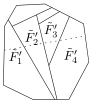
\includegraphics[width=9cm,height=6cm]{rysunki/usuniete_si.png}
  \caption{Podział płaszczyzny po usunięciu odcinka $s_i$}
\end{figure} 

Po tej operacji, każda ze ścian $F'_j$ w $F$ powiększa się w $S'$, a dodatkowe części ścian sumują się do $F$. Widzimy, że każdy z 1-nadajników rozmieszczonych wewnątrz ścian $F'_j$ pokrywa przynajmniej $F'_j$, a więc razem nadajniki $F'_1,\ldots,F'_k$ strzegą ściany $F$.

\begin{Twierdzenie} \cite{knadajniki}
  Dowolny podział gilotynowy możemy strzec przez co najwyżej $\frac{n+1}{2}$ 1-nadajników.
\end{Twierdzenie}
\begin{proof}
	Rozpatrzmy graf dualny $T$ podziału. $T$ jest triangulacją o $n + 1$ krawędziach. Niech $M$ będzie maksymalnym skojarzeniem w grafie $T$. Każda nieskojarzona krawędź jest incydentna tylko z krawędziami skojarzonymi ( w przeciwnym przypadku skojarzenie nie byłoby maksymalne). Niech $G$ będzie zbiorem 1-nadajników uzyskanych przez rozmieszczenie ich w pierwszej skojarzonej krawędzi $e \in M$. W takim wypadku |$G$| = |$M$| $\le \frac{n+1}{2}$. Dla każdej ściany $F$ z $S$, $F$ albo zawiera 1-nadajnik w $G$ albo wszystkie sąsiednie ściany, które dzielą krawędź z $F$, zawierają 1-nadajnik w $G$. W pierwszym przypadku $F$ jest oczywiście strzeżona. Natomiast w drugim przypadku, zgodnie z lematem \ref{sasiednie sciany strzega F}, ściana $F$ również jest strzeżona. Dlatego $G$ jest zbiorem 1-nadajników, które strzegą wszystkie ściany $F$ o mocy co najwyżej $\frac{n+1}{2}$
\end{proof}

\begin{figure}[ht!]
  \centering
  \label{pokrycie f}
  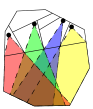
\includegraphics[width=9cm,height=6cm]{rysunki/pokrycie_f.png}
  \caption{Nadajniki każdej ze ścian strzegące całą ścianę F.}
\end{figure} 

\chapter{Strażnicy na siatkach}
\section{Siatki 2D}
W 1986 roku Simeon Ntafos przedstawił koncept strażników strzegących specjalnej klasy wielokątów - siatek.
Przez siatkę $P$ rozumiemy połączony zbiór poziomych oraz pionowych odcinków prostych (rys. \ref{fig:siatka 2d}). Możemy na nią spojrzeć jak na wielokąt prostokątny z dziurami, który składa się z bardzo cienkich korytarzy.
Widzialnością w siatce nazywamy sytuację, w której strażnik będący w punkcie \textit{x} widzi punkt \textit{y} jeżeli odcinek \textit{xy} należy do zbioru P (czyli jest korytarzem siatki).
 \begin{figure}[ht!]
   \centering
   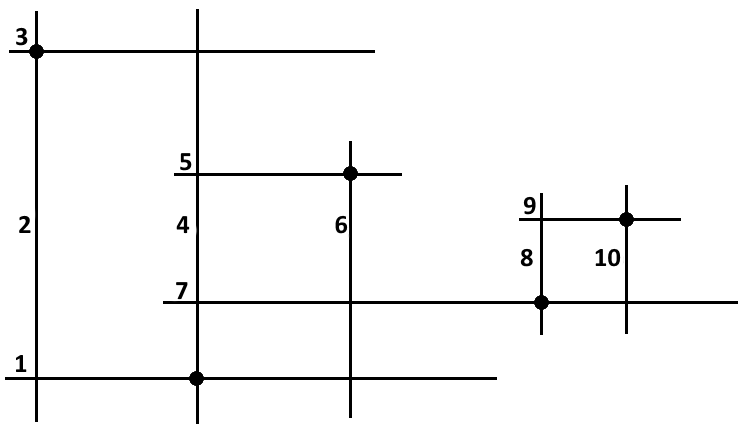
\includegraphics[width=14cm,height=6cm]{rysunki/przykladowa_siatka.png}
   \caption{Siatka strzeżona przez 6 strażników}
   \label{fig:siatka 2d}
 \end{figure} 

\begin{Twierdzenie}\cite{ntafos}
	Minimalna ilość strażników potrzebna aby \it{strzec siatkę} o $n$ odcinkach wymaga $n - m$strażników, gdzie $m$ to moc doskonałego skojarzenie w grafie przecięć, które można znaleźć w czasie $\theta(n^{2.5})$
\end{Twierdzenie}
Ntafos zaproponował elegancki algorytm aby znaleźć minimalną ilość strażników potrzebną do strzeżenia siatki.
\begin{proof}
Aby strzec całej siatki, przynajmniej jeden strażnik musi znajdować się w każdym korytarzu. Niech \textit{G} będzie grafem przecięć siatki. Każdy wierzchołek z grafu \textit{G} odpowiada odcinkowi a dwa wierzchołki są połączone krawędzią wtedy i tylko wtedy, jeżeli odpowiadające im odcinki przecinają się.
 \begin{figure}[ht!]
   \centering
   \label{fig:graf przeciec}
   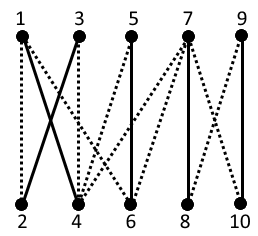
\includegraphics{rysunki/graf_skojarzen.png}
   \caption{Graf przecięć siatki. Skojarzenia oznaczono linią ciągłą.}
 \end{figure} 
 \\Skojarzeniem w grafie $G$ nazywamy zbiór krawędzi $M$ takich, że każda krawędź z $G$ jest incydentna co najwyżej z jedną krawędzią z $M$. Skojarzeniem doskonałym nazywamy takie skojarzenie, które ma maksymalną moc. W grafie przecięć \ref{fig:graf przeciec} skojarzenie to nic innego jak zbiór wszystkich przecięć korytarzy pionowych z poziomymi. Doskonałe skojarzenie dla dowolnego grafu o $V$ wierzchołkach można znaleźć w czasie O($V^{2.5}$) (Even 1979). Jako że graf $G$ jest dwudzielny ponieważ przecięcia występują tylko pomiędzy korytarzamia pionowymi i poziomymi problem znalezienia maksymalnego skojarzenia sprowadza się do problemu kojarzenia małżeństw, który da się rozwiązać w czasie O($V^{1/2}$E), gdzie $V$ to ilość wierzchołków a $E$ ilość krawędzi w grafie dwudzielnym (Even 1979). Dla siatki o $n$ odcinkach $V = n$ a maksymalna ilość krawędzi to $E = O(n^2)$ więc w najgorszym przypadku maksymalne skojarzenie znajdziemy w czasie $O(n^{2.5})$.
 \\\indent Aby strzec siatkę w całości, każdy odcinek wymaga strażnika a więc rozmieszczenie ich na przecięciach korytarzy pozwala strzec co najwyżej dwa odcinki. Stąd uzyskujemy minimalną ilość strażników wynoszącą $\ceil{\frac{n}{2}}$ dla siatki o $n$ odcinkach. Jeżeli graf posiada doskonałe skojarzenie o rozmiarze $\ceil{\frac{n}{2}}$ wtedy taka sama ilość strażników jest wystarczająca. Należy ich rozmieścić w każdym przecięciu korytarzy odpowiadającemu skojarzeniu w grafie. Jeżeli skojarzenie ma moc $m$, wtedy rozmieszczenie w odpowiadającym im przecięciach strzeże $2m$ odcinków. W każdym z pozostałych $n - 2m$ odcinków musi zostać umieszczony jeden strażnik, co w sumie daje nam $m + n - 2m = n - m$ strazników. Jest to jednocześnie dolne ograczenie: jeżeli mniej niż $n - m$ strażników wystarcza, wtedy ponad $m$ strażników musi kryć dwa odcinki a to daje nam skojarzenie o rozmiarze większym niż $m$, co nie jest możliwe.
\end{proof}

 \section{Siatki 3D}
 	Ntafos przedstawił również zagadnienie strzeżenia siatki w trzech wymiarach, które należy do klasy problemów NP-Zupełnych. Dowód uzyskamy przez redukcję problemu pokrycia wierzchołkowego grafu co najwyżej trzeciego stopnia, który należy do klasy NPC (Garey i Johnson 1979).
\begin{Definicja}
	Pokryciem wierzchołkowym grafu $G = (V,E)$ nazywamy podzbiór $V_0 \subseteq V$ takich wierzchołków grafu, że każda krawędź z $G$ jest incydentna z przynajmniej jednym wierzchołkiem $V_0$.
\end{Definicja}
Naszym celem jest stworzenie trójwymiarowej siatki $P$, którą możemy pokryć co najwyżej $g$ strażnikami wtedy i tylko wtedy jeżeli istnieje pokrycie wierzchołkowe $G$ przez co najwyżej $K$ wierzchołków.
W tym celu etykietujemy wszystkie wierzchołki grafu $G$ kolejnymi liczbami $1,2,\ldots,n = |V|$. Następnie, przypisujemy wierzchołki punktom siatki wzdłuż prostej poprowadzonej pomiędzy punktami (0,0,0) i (1,1,1) tak, aby każdy wierzchołek $i$ otrzymał punkt siatki $v_i = (3i, 3i, 3i)$. Krawędzie $G$ reprezentowane są przez linie łączące węzły siatki. Jako że każdy wierzchołek grafu $G$ jest stopnia co najwyżej trzeciego, każdej incydentnej krawędzi możemy przypisać jeden z kierunków $(x,y,z)$.
\\\indent Załóżmy teraz, że wszystkie krawędzie incydentne z wierzchołkami $1,\ldots,i-1$ grafu $G$ zostały przypisane do ścieżek siatki $P$ oraz rozpatrzmy krawędź (i,j), i < j. Przyjmujemy, że ścieżka z $v_i$ do $v_j$, dla i < j, wychodzi z $v_i$ dodatnią osią $+x$, $+y$ lub $+z$ a wchodzi do $v_j$ ujemną osią $-x$, $-y$ lub $-z$. Skoro stopień wierzchołka $i$ wynosi co najwyżej trzy, jedna z trzech osi $+x$, $+y$ lub $+z$ rozpoczynająca się w (3i, 3i, 3i) nie może zawierać żadnej ścieżki siatki $P$. Załóżmy, że oś $+x$ jest wolna. W takim wypadku połączmy $v_i = (3i, 3i, 3i)$ z $v_j = (3j, 3j, 3j)$ trzema odcinkami:
\begin{itemize}
	\item $(3i, 3i, 3i) -> (3j, 3i, 3i)$
	\item $(3j, 3i, 3i) -> (3j, 3j, 3i)$
	\item $(3j, 3j, 3i) -> (3j, 3j, 3j)$
\end{itemize}
Oczywiście, powyższe odcinki nie mogą przecinąć się z żadnymi już istniejącymi ścieżkami. Przykład takiego połączenia widać na rysunku \ref{fig:nowe sciezki}, w przypadku gdy wolna jest oś $+x$, $+y$ lub $+z$.
\begin{figure}[ht!]
  \centering
  a)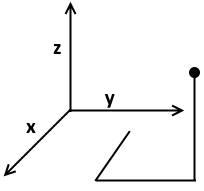
\includegraphics[width=4cm,height=5cm]{rysunki/wolne_x.png}
  b)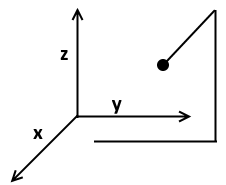
\includegraphics[width=4cm,height=5cm]{rysunki/wolne_y.png}
  c)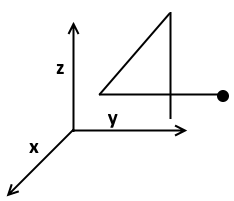
\includegraphics[width=4cm,height=5cm]{rysunki/wolne_z.png}
  \caption{Nowo powstałe ścieżki w przypadku wolnych osi $+x$, $+y$ lub $+z$}
  \label{fig:nowe sciezki}
\end{figure} 
\\\indent Zajmiemy się teraz przypadkiem, w którym fragment ścieżki pomiędzy węzłami $v_i$ i $v_j$ nakłada się ze ścieżką łącząca $v_j$ z $v_j$ wzdłuż osi $-z$, dla $k < i < j$. W takiej sytuacji przynajmniej jedna z osi $-x$ lub $-y$ musi być wolna. Jeżeli jest to oś $-x$ zmieniamy ścieżkę zgodnie z rysunkiem \ref{fig:nakladanie}a, jeżeli $-y$ wtedy musimy poprawić ścieżkę zgodnie z rysunkiem \ref{fig:nakladanie}b. Analogicznych operacji dokonamy jeżeli zajęta będzie oś $-x$ lub $-y$.
\begin{figure}[ht!]
  \centering
  a)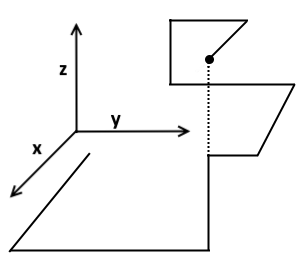
\includegraphics[width=6cm,height=5cm]{rysunki/zajete_z.png}
  b)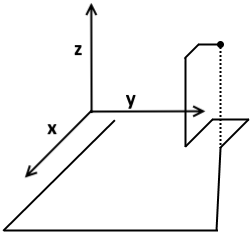
\includegraphics[width=6cm,height=5cm]{rysunki/zajete_z2.png}
  \caption{Omijanie zajętej ścieżki w przypadku wolnej osi $-x$ oraz $-y$}
  \label{fig:nakladanie}
\end{figure} 
Tak powstała konstrukcja składa się z dziewięciu krawędzi. W przypadku, gdy zajdzie potrzeba ominięcia jeszcze jednej krawędzi uzyskamy ścieżkę składającą się z 15 odcinków.
\todo{Rysunek?}
\\\indent Po stworzeniu siatki wg powyższego przepisu uzyskamy w sumie \textit{e} krawędzi grafu \textit{G} składających się ze ścieżki $e_3$ złożonej z 3 odcinków, ścieżki $e_9$ z 9 odcinków oraz ścieżki $e_{15}$ z 15 odcinków co daje nam \textit{e = $e_3$ + $e_9$ + $e_{15}$}.

\begin{Lemat}\cite{orourke}
	Pokrycie wierzchołkowe grafu \it{G} o rozmiarze \it{K} istnieje wtedy i tylko wtedy jeżeli istnieje pokrycie siatki \it{P} wg powyższego algorytmu przez \it{g = K + $e_3$ + 4$e_9$ + 7$e_{15}$} strażników.
\end{Lemat}
\begin{proof} 
	Załóżmy, że istnieje pokrycie wierzchołkowe \textit{C} grafu \textit{G} o rozmiarze \textit{K}. Następnie, rozmieśćmy strażnika w każdym przecięciu siatki $P$ która odpowiada wierzchołkowi w \textit{C}.
	Niech $p_3$ będzie ścieżką złożoną z 3 odcinków w $P$ pomiędzy $v_i$ a $v_j$. Ponieważ \textit{C} jest pokryciem wierzchołkowym, przynajmniej w jednym z węzłów $v_i$ lub $v_j$ znajduje się strażnik a więc potrzebujemy jeszcze jednego strażnika aby strzec $p_3$. Podobna sytuacja występuje dla ścieżki $p_9$ pomiędzy $v_i$ oraz $v_j$. Jeden z węzłów $v_i$ lub $v_j$ jest już strzeżony więc dodatkowo potrzebujemy 4 strażników. Dla ścieżki $p_{15}$ potrzebujemy 7 dodatkowych strażników, co w rezultacie daje nam \textit{K + $e_3$ + 4$e_9$ + 7$e_{15}$} strażników.
	\\\indent Załóżmy teraz, że aby strzec siatkę $P$ wystarczy \textit{K + $e_3$ + 4$e_9$ + 7$e_{15}$} strażników. Każda z trzy elementowych ścieżek $e_3$ wymaga jednego strażnika w wewnętrznym rogu. Ścieżka złożona z dziewięciu odcinków wymaga czterech strażników rozmieszczonych w wewnętrznych rogach a piętnastowa odcinkowa - siedmiu. Stąd uzyskujemy sumę $e_3$ + 4$e_9$ + 7$e_{15}$ strażników rozmieszczonych w miejscach innych niż punkty siatki, którym odpowiadają wierzchołki grafu \textit{G}. Pozostało nam jeszcze \textit{K} strażników, których możemy umieścić tylko w punktach siatki odpowiadających wierzchołkom grafu \textit{G}. Załóżmy więc, że strażnicy rozmieszczeni w tych punktach nie należą do pokrycia wierzchołkowego \textit{G}. W takim wypadku krawędź \textit{(i, j)} z \textit{G} nie jest incydentna z żadnym wierzchołkiem należącym do pokrycia wierzchołkowego a więc odpowiadająca jej ścieżka w siatce $P$ nie posiada strażników zarówno w $v_i$ ani w $v_j$. Wiemy jednak, że aby pokryć np. ścieżkę trójelementową jeden strażnik w wewnętrznym rogu jest w stanie strzec tylko dwa z trzech odcinków. Analogiczna sytuacja występuje dla ścieżek o długości dziewięciu oraz piętnastu odcinków, w których, odpowiednio, czterech i siedmiu strażników jest w stanie strzec co najwyżej osiem i czternaście z dziewięciu oraz piętnastu odcinków. Stąd wnioskujemy, że jeżeli \textit{K} strażników nie stanowi pokrycia wierzchołkowego to nie możemy pokryć siatki $P$ przez \textit{K + $e_3$ + 4$e_9$ + 7$e_{15}$} strażników a więc \textit{K} strażników musi być pokryciem wierzchołkowym o rozmiarze co najwyżej \textit{K}. 
\end{proof}

\begin{Twierdzenie}\cite{ntafos}
	Zagadnienie strzeżenia trójwymiarowej siatki przez minimalną ilość strażników należy do klasy problemów NP-zupełnych.
\end{Twierdzenie}
\begin{proof} 
	Ponieważ strażnicy mogą być rozmieszczeni tylko na skrzyżowania siatki lub w jej rogach, których jest skończona liczba rozwiązanie możemy zgadnąć oraz sprawdzić w czasie wielomianowym. Problem pokrycia wierzchołkowego należy do klasy NP-zupełnej a więc zagadnienie zredukowanie do tego problemu również należy do klasy NP-zupełnej.
\end{proof}

\chapter{Problem pościgu i ucieczki w grafie}
\section{Gra w złodzieja i policjanta}
Mając dany graf \textit{G}, zbiór reguł \textit{S}, liczbę całkowita \textit{k}, oraz dwa warunki \textit{$T_1$, $T_2$}, gra zaczyna się od rozmieszczenia przez gracza pierwszego (policjanta) nie więcej niż \textit{k} żetonów na wierzchołkach grafu \textit{G}. Gracz numer dwa (złodziej) rozmieszcza jeden żeton na dowolnym wierzchołku \textit{G}. Następnie gracze przesuwają swoje żetony, zgodnie z regułami \textit{S}, dopóki nie zajdzie jeden z warunków $T_i$. Jeżeli końcowa konfiguracja spełnia warunek $T_1$ - wygrywa policjant, w przeciwnym wypadku wygrywa złodziej. W klasycznej wersji gry, obaj gracze znają rozmieszczenie wszystkich żetonów a jedynym warunkiem końcowym jest aby żeton gracza pierwszego oraz drugiego znajdował się na tym samym wierzchołku grafu G.
Reguły \textit{S} wyglądają następująco:
\begin{enumerate}
  \item Gracze wykonują ruchy na przemian
  \item Gracz pierwszy w swojej kolejce może odmówić ruchu lub przesunąć wzdłuż krawędzi jeden ze swoich żetonów na wierzchołek sąsiedni z aktualnie zajmowanym
  \item Gracz drugi w swojej kolecje może odmówić ruchu lub przesunąć wzdłuż krawędzi swój żeton na wolny wierzchołek, sąsiedni z wierzchołkiem aktualnie zajmowanym
\end{enumerate}

Problem ma praktyczne zastosowanie na przykład w planowaniu ruchu robotów, kiedy ważnym jest aby nie następowały kolizje lub poważniejsze zderzenia.

Zagadnienie pościgu i ucieczki w grafie, opiera się na przeszukiwaniu grafu w taki sposób aby po wykonaniu \textit{n} kroków, policjant zauważył złodzieja (tzn. znajdował się w tym samym wierszu lub w tej samej kolumnie) lub, w trudniejszym wariancie, znajdował się w tym samym wierzchołku co złodziej. Taką sytuację uznajemy za zwycięstwo goniącego, w przeciwnym wypadku zwycięża złodziej. Obaj uczestnicy poruszają się tylko po wierszach i kolumnach siatki z ograniczoną prędkością.

Najprostszym przykładem gry, w której zawsze zwycięża policjant jest drzewo oraz współczynnik k = 1. W takim przypadku policjant w każdym kolejnym ruchu zbliża się do drugiego gracza, który w żadnym momencie nie jest w stanie go minąć, co zawsze prowadzi do zwycięstwa goniącego.

\subsection{Wariant Sugiharu i Suzuki}
W tym rozdziale zajmę się innym wariantem gry, przedstawionym przez Sugiharu i Suzuki, w którym warunkiem zwycięstwa policjanta jest zauważenie złodzieja a gra odbywa się na grafie \textit{G} przypominającym prostokątną siatkę.
Przez siatkę rozumiemy graf \textit{$G_{n,m}$}, gdzie \textit{n} to liczba wierzchołków a \textit{m} liczba krawędzi, z których każda ma długość jeden. Zakładamy również, że graf jest rozpięty na płaszczyźnie z punktem poczatkowym \textit{$v_{0,0}$} w lewym górnym wierzchołku.
\begin{Definicja}
  Gracz A \it{jest widoczny} dla gracza B wtedy i tylko wtedy, gdy obaj znajdują się w tej samej kolumnie lub w tym samym wierszu siatki, niezależnie od odległości która ich dzieli.
\end{Definicja}

Gracz przesuwają swoje żetony tylko po krawędziach grafu a szybkość ruchu jest określona przed rozpoczęciem gry.
W tym wariancie gry, gracze nie mają całkowitej wiedzy o pozycjach, które zajmują. Tylko złodziej posiada wszystkie informacje o miejscach, które zajmuje policjant. Ścigający za to nie wie nic o pozycji uciekającego, dopóki nie zostanie on zauważony. Dodatkowo, ruchy pierwszego gracza są z góry określone, zanim gra w ogóle się rozpocznie.
Zasady \textit{S} wyglądają następująco:
\begin{enumerate}
  \item Gracze poruszają się w czasie rzeczywistym
  \item Prędkość ścigającego jest stała i wynosi $s_n$
  \item Uciekający porusza się z prędkością co najwyżej $s_c$
\end{enumerate}

Warunki kończące grę:
\begin{enumerate}
  \item Złodziej został zauważony przez policjanta
  \item Uciekający zawsze jest w stanie zapobiec zwycięstwu policjanta
\end{enumerate}

Podobnie jak zwykły problem gonitwy i ucieczki, również ta odmiana jest całkowicie deterministyczna i zależy od parametrów początkowych gry. Naszym celem jest określenie warunków, w których zawsze zwycięża gracz pierwszy. 

\begin{Twierdzenie} \cite{poscig}
	Jeżeli $S_n$ $\le$ n + 1, policjant zawsze wygrywa dla stałej $S_c$ = n + 1.
\end{Twierdzenie}
\begin{proof}
	Aby dowieść powyższego twierdzenia skorzystamy z następującego algorytmu
	\begin{enumerate}
		\item Gracz pierwszy porusza się w dół kolumną \textit{j}, startując w wierzchołku \textit{(0,j)}, przechodząc przez wierzchołek \textit{(n, j)} a kończąc ruch w \textit{(n, j + 1)}. Pokonanie takiej trasy zajmuje jedną jednostkę czasu.
		\item Następnie, przesuwa się w górę kolumną \textit{j + 1}, kończąc ruch w wierzchołku \textit{(0,j)}. Pokonanie takiej ścieżki również zajmuje jedną jednostkę czasu.
		\item Powtarzamy ruch nr 1
		\item Wykonuje ruch w górę kolumną \textit{j + 1}, kończąc go w wierzchołku \textit{(0,j + 1)}, tracąc $\frac{n}{n+1}$ jednostki czasu.
	\end{enumerate}
	\begin{figure}[ht!]
	  \centering
	  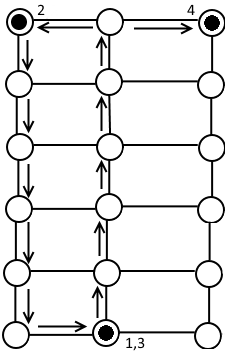
\includegraphics[height=6cm]{rysunki/schemat_ruchu.png}
	  \caption{Trasa pokonana przez gracza pierwszego w wyniku algorytmu}
	  %\todo[inline]{Poprawić ten obrazek}
	\end{figure} 

	Czas, którego potrzebował gracz pierwszy aby wykonać powyższy schemat wynosi $t_{j+1}$ = $t_j$ + 3 + $\frac{n}{n+1}$.
	Zakładamy, że po wykonaniu powyższych ruchów, gracz numer dwa albo został już zauważony, co kończy grę, lub znajduje się w części siatki ograniczonej przez wierzchołki [(0,0), (n, j + 1)].
	\indent Jako że gra toczy się dalej, gracz numer dwa nie może znajdować się w pierwszym wierszu ani \textit{j-tej} kolumnie ponieważ wtedy byłby widoczny dla policjanta. W czasie \textit{$t_j$} drugi gracz znajduje się w części siatki ograniczonej przez wierzchołki [(0,j), (n, j + 1)] i próbuje się przedostać do części [(0,0), (n, j + 1)]

	\begin{figure}[ht!]
	  \centering
	  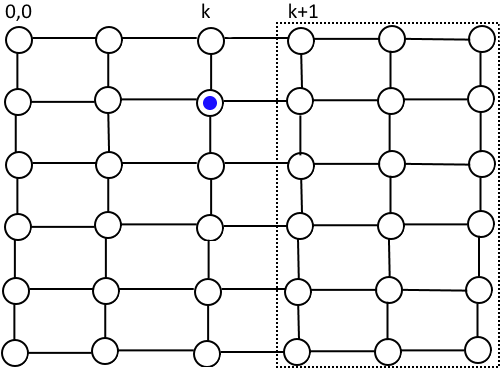
\includegraphics[height=5cm]{rysunki/podsiatka.png}
	  \caption{Złodziej znajduje się w części siatki zaznaczonej linią przerywaną}
	\end{figure} 

	\indent W czasie, kiedy policjant przemieszcza się kolumną \textit{j}, złodziej może zbliżać się do niej wierszem \textit{i}. Policjant dotrze do wierzchołka (i,j) po czasie $\frac{i}{n+1}$ a więc do tego momentu złodziej musi znajdować się powyżej (lub poniżej) wiersza \textit{i}. Wynika z tego, że w momencie kiedy gracz nr jeden kończy pierwszy ruch, drugi gracz znajduje się w odległości $\frac{1-i}{n+1}$ - $\epsilon$ pomiędzy kolumną (i,j + 1) a kolumną (i,j). Obrazuje to rysunek \ref{fig:pierwszy krok}.
	\begin{figure}[ht!]
	  \centering
	  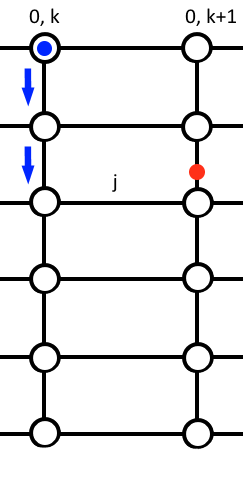
\includegraphics[width=5cm,height=5cm]{rysunki/poscig_1.png}
	  \caption{Pierwszy etap pościgu.}
	  \label{fig:pierwszy krok}
	\end{figure}
	\\\indent Pierwszy gracz ponownie przekroczy wiersz \textit{i} w drugim kroku algorytmy po upływie $\frac{n-1}{n+1}$ czasu. Do tego momentu, drugi gracz musi przejść cały wiersz i znaleźć się w kolumnie \textit{j}. Żeby tego dokonać musi przemieścić się o $\frac{i}{n+1}$ + $\delta$ w ciągu $\frac{n-1}{n+1}$ jednostek czasu. Daje nam to ograniczenie \textit{i < $\frac{n}{2}$}.
	\\\indent Pomiędzy momentem kiedy policjant przekracza wiersz \textit{i} w kroku drugim a przejściem do wierzchołka (0,j) mija $\frac{i}{n+1}$ jednostki czasu. W sumie mijają dwie jednostki czasu od momentu $t_j$. Złodziej startując w kolumnie \textit{j + 1} i poruszając się wzdłuż wiersza \textit{i} nie ma wystarczajaco dużo czasu aby przesunąć się do wiersza \textit{i - 1} lub \textit{i + 1} ponieważ nie może rozpocząć ruchu dopóki pierwszy gracz nie przekroczy wiersza \textit{i}. Więc w momencie, kiedy ścigający kończy ruch nr dwa, drugi gracz musi znajdować się w odległości nie większej niż $\frac{i}{n+1}$ - $\gamma$ od (i,j). Jako że \textit{i < $\frac{n}{2}$}.
	\begin{center}
	$\frac{i}{n+1}$ - $\gamma$ < 1 - $\frac{i}{n+1}$
	\end{center}
	Widać to na poniższym rysunku.
	\begin{figure}[ht!]
	  \centering
	  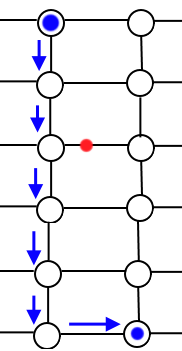
\includegraphics[width=5cm,height=5cm]{rysunki/poscig_2.png}
	  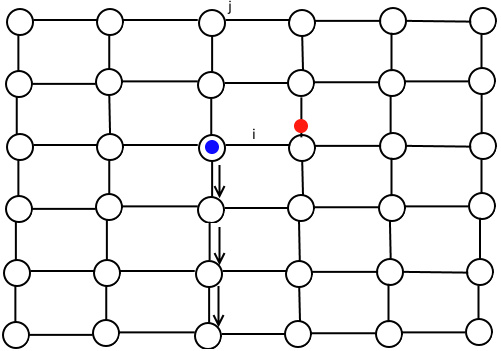
\includegraphics[width=5cm,height=5cm]{rysunki/poscig_3.png}
	  \caption{Drugi etap pościgu}
	  \label{fig:drugi krok}
	\end{figure}

	\indent Pierwszy gracz osiąga (i,j) w kroku trzecim po upływie kolejnych $\frac{i}{n+1}$ jednostek. W tym samym czasie drugi gracz nie jest w stanie osiągnąć kolumny \textit{j - 1} ani wrócić do \textit{j + 1} a więc zostaje zauważony.
	\begin{figure}[ht!]
	  \centering
	  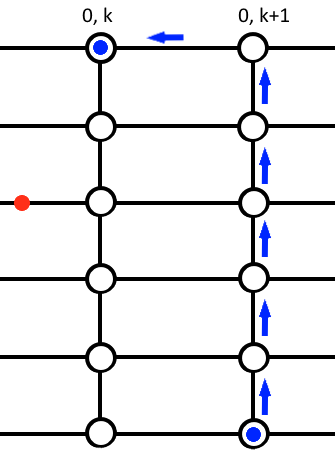
\includegraphics[width=5cm,height=5cm]{rysunki/poscig_4.png}
	  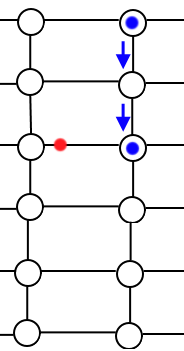
\includegraphics[width=5cm,height=5cm]{rysunki/poscig_5.png}
	  \caption{Ostatni etap pościgu.}
	  \label{fig:ostatni etap poscigu}
	\end{figure} 

	\indent Ponieważ policjant widzi przez całą długość wiersza/kolumny, takie samo rozumowanie będzie miało zastosowanie jeżeli złodziej będzie rozpoczynał swój ruch z każdej kolumny \textit{k > j + 1}. W ten sposób jeżeli pierwszy gracz rozpocznie grę w punkcie (0,0) oraz wszystkie założenia początkowe będą spełnione zawsze zakończy grę sukcesem w czasie nie większym niż \textit{$t_n$}.
\end{proof} 
\summary
Kiedy Klee po raz pierwszy sformułował problem galerii sztuki na pewno nie spodziewał się jak wielka ilość zagadnień zrodzi się z tego stosunkowo prostego pomysłu. 
% Streszczenie…

% % załączniki (opcjonalnie):
\appendix
\chapter{Triangulacja wielokąta}\label{triangulacja}
\begin{Lemat}\label{podzial na trojkaty}
$N$-kąt prosty można zawsze podzielić na $n-2$ trójkątów.
\end{Lemat}
\begin{proof}
	Dowód przez indukcję po n.
	\\Jeżeli n = 3, to wielokąt jest już podzielony $3 - 2 = 1$ trójkąt.
	Załóżmy, że n $\ge$ 3 i rozpatrzmy skrajny lewy wierzchołek \textit{v} oraz jego sąsiadów \textit{u}, \textit{w}.
	W pierwszym przypadku odcinek \textit{uw} jest przekątną, a w drugim część krawędzi wielokąta P leży wewnątrz trójkąta \textit{uvw}.
	\begin{align*}
	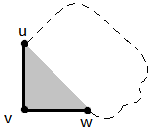
\includegraphics[height=5cm]{rysunki/triangulacja_1.png} \hspace{3cm} 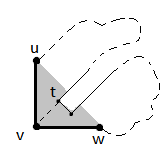
\includegraphics[height=5cm]{rysunki/triangulacja_2.png}
	\end{align*}
	\\\indent W pierwszym przypadku przekątna $\overline{u w}$ dzieli wielokąt na trójkąt oraz wielokąt prosty o $n - 1$ wierzchołkach, na których wykonujemy krok indukcyjny, otrzymując $1 + (n - 1) -2 = n - 2$ trókątów, najbliższych do $v$.
	\\\indent W przypadku drugim znajdujemy punkt $t$, który znajduje się najdalej od prostej $uw$, a następnie łączymy go z punktem $v$. Odcinek $\overline{v t}$ musi być przekątną, która dzieli wielokąt na dwa proste wielokąty o $m$ oraz $n - m + 2$ wierzchołkach, gdzie $3 \ge m \ge n-1$ na których wykonujemy krok indukcji: z założenia indukcyjnego, podział wielokąta skłąda się z $(m - 2) + ((n - m + 2) -2) = n - 2$ trójkątow.
\end{proof}

% %Załącznik…
% %
% %\chapter{Tytuł załącznika}
% %
% %Załącznik…
\begin{bibdiv}
\begin{biblist}
 \bibitem{orourke} Joseph O'Rourke, Art gallery theorems and algorithms (1987)
 \bibitem{chvatal} Victor Chv\'atal, A combinatorial theorem in plane geometry, Journal of Combinatorial Theory 18, 39-41 (1975)
 \bibitem{guarding walls} Aldo Laurentini, Guarding the walls of an art gallery (The Visual Computer, 1999)
 \bibitem{czyzowicz} J. Czyzowicz, E. Rivera-Campo, N. Santoro, J. Urrutia i J. Zaks, Guarding rectangular art galleries. Discrete Applied Math, 50:149–157, 1994. 
 \bibitem{illumination} Jorge Urrutia, Art gallery and illumination problems (2004)
 \bibitem{knadajniki} Brad Ballinger, Nadia Benbernou, Prosenjit Bose, Mirela Damian, Erik D. Demaine,Vida Dujmovi\`c, Robin Flatland, Ferran Hurtado, John Iacono, Anna Lubiw, Pat Morin, Vera Sacristán, Diane Souvaine i Ryuhei Uehara, Coverage with k-transmittes in the presence of obstacles (?)
 \bibitem{poscig} Robin W. Dawes, Some pursuit - evasion problems on grid
 \bibitem{fisk} Steve Fisk, A short proof of Chv\'atal's watchman theorem (1977), Journal of Combinatorial Theory 24, 374 
 \bibitem{tutte} Tutte, W. T. "The Factorization of Linear Graphs." J. London Math. Soc. 22, 107-111, 1947.
 \bibitem{ntafos} Simeon Ntafos, On gallery watchmen in grids, Information Processing Letters Volume 23, Issue 2, 20 August 1986, Pages 99–102
\end{biblist}
\end{bibdiv}

% spis rysunków
\listoffigures

% \oswiadczenie

\end{document}